\section{Ejercicios resueltos}
\subsection{Tema 1: Fundamentos y propiedades de los fluidos}
\begin{enumerate}
	\item Obtener el ángulo de mojabilidad $\theta_c$ 
	\begin{figure}[H]
		\begin{minipage}{0.7\textwidth}
		\centering
		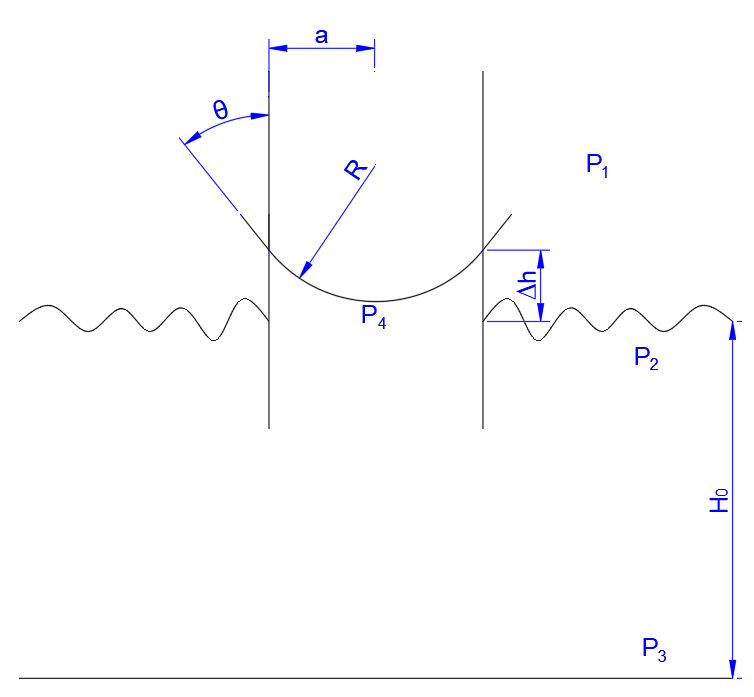
\includegraphics[width=0.7\linewidth]{imagenesEjercicios/mojabilidad}
		\caption{Esquema del problema.}
		\label{fig:mojabilidad}
	\end{minipage}%
	\begin{minipage}{0.3\textwidth}
	\[\textcolor{blue}{P_2=P_1=P_a}\]
	\[\textcolor{blue}{P_2=\rho g H_0=P_3}\]
	\[\textcolor{blue}{P_3=P_4+\rho g (H_0+\Delta h)}\]
	\[\textcolor{blue}{P_1-P_4=\frac{2\sigma}{R}}\]
	\[\textcolor{blue}{\frac{2\sigma}{R}=\rho g \Delta h}\]
	\[\textcolor{blue}{Rcos(\theta_c)=a}\]
	\[\textcolor{blue}{\theta_c=arccos\left(\frac{a\rho g \Delta h}{2\sigma}\right)}\]
	
	\end{minipage}
	\end{figure}
	
	\item En el pueblo de Aisa se ha instalado un nuevo sistema de presión para el abastecimiento
	de agua del municipio. El agua procedente de un manantial es impulsado por una bomba
	y se almacena en un depósito sobrepresor. Para controlar la presión del agua a la entrada
	y salida de la bomba se han montado un vacuómetro y un manómetro en los puntos de
	interés. Cuando el vacuómetro marca 0.75 bares y el manómetro marca 4.2 bares, ¿cuál
	será el valor de la presión absoluta?. ¿Existe riesgo de cavitación en algún punto de la
	conducción?. Datos: $p_{atm}$ = 816,91 hPa; $p_v$=159856 Pa.
	\begin{figure}[H]
		\begin{minipage}{0.7\textwidth}
		\centering
		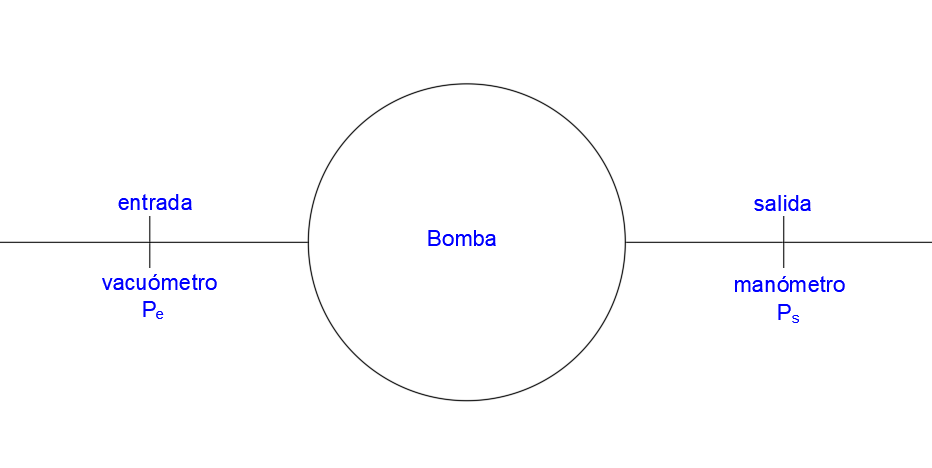
\includegraphics[width=0.7\linewidth]{imagenesEjercicios/bombaAisa}
		\caption{Esquema bomba de agua.}
		\label{fig:bombaaisa}
	\end{minipage}%
	\begin{minipage}{0.3\textwidth}
	\[\textcolor{blue}{P_v=P_{atm}-P_e}\]
	\[\textcolor{blue}{P_m=P_s-P_{atm}}\]
\[ \textcolor{blue}{P_e=81691-75000=6691 Pa}\]
\[\textcolor{blue}{P_s=81691+420000=501691 Pa}\]
\textcolor{blue}{Existe cavitación a la entrada.}
	
	\end{minipage}
\end{figure}

	\newpage
	\item La presión en un punto de un fluido ($\rho = 1234 \frac{kg}{m^3}$) alcanza el valor de 3 bares. Expresar
	el valor de la presión en milímetros de mercurio (cm Hg) y en columna de metros de agua
	(m.c.a.). Datos: $\rho_{Hg,rel} = 13,6$
	\[\textcolor{blue}{\rho = 1234 \frac{kg}{m^3}}\]
	\[\textcolor{blue}{P=3\cdot10^5 Pa}\]
	\[\textcolor{blue}{1mmHg=\rho_{Hg}g h=13.6\cdot10^3\frac{kg}{m^3} \cdot9.8 \frac{m}{s^2}\cdot10^{-3}m=133.416Pa} \]
	\[\textcolor{blue}{1mca=\rho_{H_2O}g h=10^3\frac{kg}{m^3}\cdot9.8 \frac{m}{s^2}\cdot1m=9810Pa}\]
	\item Sobre una superficie de 4000 $cm^2$, orientada en el espacio por su vector normal $\vec{n}=\vec{k}$, está
	actuando una fuerza$\vec{F}=2\vec{i}+3\vec{j}-3\vec{k}$ (N). Calcular la componente normal de la fuerza y
	la presión que está soportando la superficie
		\[\textcolor{blue}{S=4000 cm^2=0.4 m^2}\]
	\[\textcolor{blue}{\vec{n}=\vec{k}}\]
	\[\textcolor{blue}{\vec{F}=2\vec{i}+3\vec{j}-3\vec{k} \rightarrow F_n=3N}\]
	\[\textcolor{blue}{P=\frac{F_n}{S}=\frac{3 N}{0.4 m^2}=7.5Pa}\]
	
	\item Sabiendo que un fluido tiene una densidad de 0.627 $\frac{kg}{l}$ y que su coeficiente de viscosidad
	absoluta es 1.2 cP, calcular su viscosidad cinemática. ¿Cuál es su densidad relativa si
	consideramos el agua como fluido de referencia?. Datos $\rho_{agua} = 999,8\frac{kg}{m^3}$
\[\textcolor{blue}{\nu = \frac{\mu}{\rho}=\frac{1.2 cP \cdot \frac{10^{-3} Pa \cdot s}{1 cP}}{0.627 \frac{kg}{l}\cdot\frac{10^3 l}{m^3}}=1.91\cdot10^{-6}\frac{m^2}{s}}\]
\[\textcolor{blue}{\rho_{rel}=\frac{\rho}{\rho_{H_2O}}=\frac{0.627 \frac{kg}{l}\cdot\frac{10^3 l}{m^3}}{999.8 \frac{kg}{m^3}}=6.27\cdot10^{-1}}\]
	
	\newpage
	\item En la Figura se muestra un bloque, de bases paralelas con dimensiones 0,3 m x 0,6
	m y altura 0,1 m, de densidad 1800 $\frac{kg}{m^3}$, que desliza con una velocidad constante de
	1 $\frac{m}{s}$ a la largo de un plano inclinado debido a la acción de las fuerzas gravitacionales
	tangenciales al mismo. Entre dicho plano y el bloque hay una película de aceite de espesor
	1 mm. Aplicando equilibrio de fuerzas, calcular la viscosidad del aceite en Po.
	\begin{figure}[H]
		
		\centering
		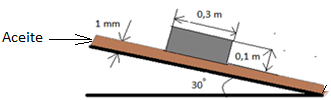
\includegraphics[width=0.7\linewidth]{imagenesEjercicios/bloqueDeslizantoT1}
		\caption{Esquema del bloque deslizando por el plano inclinado.}
		\label{fig:bloquedeslizantot1}
	\end{figure}
	\[\textcolor{blue}{F_n=m g sen\alpha}\]
	\[\textcolor{blue}{F_n=\rho V g sen\alpha}\]
	\[\textcolor{blue}{\tau=\mu\frac{v}{e}=\frac{F_n}{S}=\rho h g sen\alpha}\]
	\[\textcolor{blue}{\mu=\frac{e\rho h g sen\alpha}{v}=\frac{10^-3m\cdot1800\frac{kg}{m^3}\cdot0.1m\cdot 9.81 \frac{m}{s^2} \cdot sen(\ang{30})}{1\frac{m}{s}}=0.8829Pa\cdot s\frac{1 P}{0.1 Pa \cdot s}=8.83P}\]
\end{enumerate}
\newpage
\subsection{Tema 2: Cinemática de la partícula fluida}
\begin{enumerate}
	\item Dado el campo de velocidades de un flujo
	\[\vec{v}=4cos(\omega t)x\vec{i}-2cos(\omega t)y\vec{j}-2cos(\omega t)z\vec{k}\]
	\begin{enumerate}
		\item Indicar el tipo de flujo\\
		\textcolor{blue}{Flujo tridireccional, tridimensional y transitorio.}
		\item La ecuación de la trayectoria si en $t=0s$ se encuentra en $(x_0,y_0,z_0)$
		\[\textcolor{blue}{\vec{v}=\frac{d\vec{r}}{dt} \rightarrow \vec{r}=x\vec{i}+y\vec{j}+z\vec{k}}\]
		\[\textcolor{blue}{v_x=4cos(\omega t)x=\frac{dx}{dt}}\]
		\[\textcolor{blue}{v_y= -2cos(\omega t)y = \frac{dy}{dt}}\]
		\[\textcolor{blue}{v_z= -2cos(\omega t)z = \frac{dz}{dt}} \]
		\[\textcolor{blue}{\ln x|_0^t=\left.{\frac{4sen(\omega t)}{\omega}}\right |_0^t \rightarrow x=x_0 e^{\frac{4sen(\omega t)}{\omega}}}\]
		\[\textcolor{blue}{y=y_0 e^{\frac{-2sen(\omega t)}{\omega}}}\]
		\[\textcolor{blue}{z=z_0 e^{\frac{-2sen(\omega t)}{\omega}}}\]
		\item La ecuación de las sendas
		\[\textcolor{blue}{\ln \frac{x}{x_0}=\frac{4sen(\omega t)}{\omega}}\]
		\[\textcolor{blue}{\ln \frac{y}{y_0}=\frac{-2sen(\omega t)}{\omega}}\]
		\[\textcolor{blue}{\ln \frac{z}{z_0}=\frac{-2sen(\omega t)}{\omega}}\]
		\[\textcolor{blue}{\frac{1}{2}\ln \frac{x}{x_0}=-\ln \frac{y}{y_0} \rightarrow xy^2=x_0y_0^2}\]
		\[\textcolor{blue}{\ln \frac{y}{z_0}=\ln \frac{y}{y_0} \rightarrow yz_0=zy_0}\]
		\item Las líneas de corriente en un instante t
		\[\textcolor{blue}{\frac{dz}{v_z}=\frac{dy}{v_y}=\frac{dx}{v_x}}\]
		\[\textcolor{blue}{\frac{dy}{-2cos(\omega t)y}=\frac{dz}{-2cos(\omega t)z}\rightarrow \frac{dy}{y}=\frac{dz}{z}\rightarrow \ln z = \ln y + C_0 \rightarrow z=C_{00}y}\]
		\[\textcolor{blue}{\frac{dy}{-2cos(\omega t)y}=\frac{dx}{4cos(\omega t)x}\rightarrow -\frac{dy}{y}=\frac{dx}{2x}\rightarrow -\ln y = \frac{1}{2}\ln x + C_1 \rightarrow C_{11}=xy^2 }\]
	\end{enumerate}
	\item La velocidad de un fluido se encuentra definida por $\vec{v}=y\vec{j}+\left(ye^{-t}-z\right)\vec{k}$ Se pide:
	\begin{enumerate}
		\item Las componentes de la velocidad 
		\[\textcolor{blue}{v_x=0} \]
		\[	\textcolor{blue}{ v_y=y}\] 
			\[\textcolor{blue}{ v_z=ye^{-t} -z}\]
		\item Caracterización del flujo\\
		\textcolor{blue}{Flujo bidireccional, bidimensional y transitorio.}
		\item La aceleración de la partícula fluida cuando en t=0s pasa por el punto (0,1,0)
			\[\textcolor{blue}{a_L=\frac{\partial\vec{v}}{\partial t}=-ye^{-t}\vec{k}}\]
		\[\textcolor{blue}{a_c=\left(\vec{v}\cdot\vec{\nabla}\right)\vec{v}=
			\left(v_x\frac{\partial}{\partial x}
			+
			v_y\frac{\partial}{\partial y}
			+
			v_y\frac{\partial}{\partial z}
			\right)\cdot
			\left(v_x\vec{i}+v_y\vec{j}+v_z\vec{k}\right)		
		}\]
		\[\textcolor{blue}{a_c=\left(v_y\frac{\partial v_y}{\partial y} + v_z\frac{\partial v_y}{\partial z} \right)
			+\left(v_y\frac{\partial v_z}{\partial y} + v_z\frac{\partial v_z}{\partial z} \right)
			= y\vec{j}+z\vec{k}
		}\]
		\[	\textcolor{blue}{
			a_T=\frac{D\vec{v}}{Dt}=\frac{\partial\vec{v}}{\partial t}+\left(\vec{v}\cdot\vec{\nabla}\right)\vec{v}=a_L+a_c=y\vec{j}+\left(-ye^{-t}+z\right)\vec{k}
		}
		\]
	\[	\textcolor{blue}{
		\left.a_T \right|_{\vec{r}=(0,1,0)m,t=0s}=\vec{j}-\vec{k} \ \frac{m}{s^2}
	}
	\]
		\item Movimiento de la partícula fluida
				\setlength{\arraycolsep}{1.5pt}
		\renewcommand{\arraystretch}{1.5}
		\[\textcolor{blue}{\overline{\overline{\xi}}=\begin{bmatrix}
				\frac{\partial v_x}{\partial x} & \frac{1}{2}\left(\frac{\partial v_x}{\partial y}+\frac{\partial v_y}{\partial x}\right) &  \frac{1}{2}\left(\frac{\partial v_x}{\partial z}+\frac{\partial v_z}{\partial x}\right)\\
				\frac{1}{2}\left(\frac{\partial v_x}{\partial y}+\frac{\partial v_y}{\partial x}\right) & \frac{\partial v_y}{\partial y} &\frac{1}{2}\left(\frac{\partial v_y}{\partial z}+\frac{\partial v_z}{\partial y}\right)\\		
				\frac{1}{2}\left(\frac{\partial v_x}{\partial z}+\frac{\partial v_z}{\partial x}\right)  &\frac{1}{2}\left(\frac{\partial v_y}{\partial z}+\frac{\partial v_z}{\partial y}\right)& \frac{\partial v_z}{\partial z}\\	
			\end{bmatrix}=
			\begin{bmatrix}
				0 & 0 &  0\\
				0 & 1 &  \frac{e^{-t}}{2}\\
				0 &  \frac{e^{-t}}{2} &  -1\\	
			\end{bmatrix}
		}\]
		\setlength{\arraycolsep}{1.5pt}
		\renewcommand{\arraystretch}{1.5}
		\[\textcolor{blue}{\overline{\overline{\gamma}}=\begin{bmatrix}
				0 & \frac{1}{2}\left(\frac{\partial v_x}{\partial y}-\frac{\partial v_y}{\partial x}\right) &  \frac{1}{2}\left(\frac{\partial v_x}{\partial z}-\frac{\partial v_z}{\partial x}\right)\\
				-\frac{1}{2}\left(\frac{\partial v_x}{\partial y}-\frac{\partial v_y}{\partial x}\right) & 0 &\frac{1}{2}\left(\frac{\partial v_y}{\partial z}-\frac{\partial v_z}{\partial y}\right)\\		
				-\frac{1}{2}\left(\frac{\partial v_x}{\partial z}-\frac{\partial v_z}{\partial x}\right)  &-\frac{1}{2}\left(\frac{\partial v_y}{\partial z}-\frac{\partial v_z}{\partial y}\right)& 0\\	
			\end{bmatrix}=
			\begin{bmatrix}
				0 & 0 &  0\\
				0 & 0 &  -\frac{e^{-t}}{2}\\
				0 &  \frac{e^{-t}}{2} &  0\\	
			\end{bmatrix}
		}\]
		
		\item ¿Podría tratarse de un líquido?
			\[\textcolor{blue}{traza(\overline{\overline{\xi}})=1-1=0\rightarrow \text{Es un líquido.} }\]
		\item La velocidad de deformación lineal específica en la dirección del vector unitario $\vec{l}=\frac{1}{\sqrt{3}}\left(\vec{i}-\vec{j}+\vec{k}\right)$
		\[\textcolor{blue}{
			\overline{\overline{\xi}}\cdot\vec{n}=\begin{bmatrix}
				0 & 0 &  0\\
				0 & 1 &  \frac{e^{-t}}{2}\\
				0 &  \frac{e^{-t}}{2} &  -1\\	
			\end{bmatrix} \cdot \frac{1}{\sqrt{3}}\begin{bmatrix}
			1 \\
			-1 \\
			1 \\	
			\end{bmatrix}=\frac{1}{\sqrt{3}}\begin{bmatrix}
			0 \\
			-1+ \frac{e^{-t}}{2}\\
			-1-  \frac{e^{-t}}{2}\\	
			\end{bmatrix}
		}\]
	\end{enumerate}
	\item Considere el flujo definido por $v_y=z\left(t+2t^2\right)$ y $v_z=2y$. Determine:
	\begin{enumerate}
		\item Tipo de flujo\\
		\textcolor{blue}{Flujo bidireccional, bidimensional y transitorio.}
		\item La aceleración de la partícula fluida: total, local, convectiva y las contribuciones de la aceleración convectiva
	
			\[\textcolor{blue}{a_L=\frac{\partial\vec{v}}{\partial t}=z(1+4t)\vec{j}}\]
			\[\textcolor{blue}{a_c=\left(\vec{v}\cdot\vec{\nabla}\right)\vec{v}=
			\left(v_x\frac{\partial}{\partial x}
			+
		v_y\frac{\partial}{\partial y}
			+
		v_y\frac{\partial}{\partial z}
			\right)\cdot
			\left(v_x\vec{i}+v_y\vec{j}+v_z\vec{k}\right)		
			}\]
			
			\[\textcolor{blue}{a_c=\left(v_y\frac{\partial v_y}{\partial y} + v_z\frac{\partial v_y}{\partial z} \right)
				+\left(v_y\frac{\partial v_z}{\partial y} + v_z\frac{\partial v_z}{\partial z} \right)
				= 2y(t+2t^2)\vec{j}+2z(t+2t^2)\vec{k}
			}\]
			\[	\textcolor{blue}{
				a_T=\frac{D\vec{v}}{Dt}=\frac{\partial\vec{v}}{\partial t}+\left(\vec{v}\cdot\vec{\nabla}\right)\vec{v}=a_L+a_c=\left[z(1+4t)+2y(t+2t^2)\right]\vec{j}+2z(t+2t^2)\vec{k}
			}
			\]
			\[\textcolor{blue}{a_{c_v}=\vec{\nabla}\frac{|\vec{v}|^2}{2}=\frac{1}{2}\left[
				\frac{\partial}{\partial x}\left(v_x^2+v_y^2+v_z^2\right)\vec{i}
				+
				\frac{\partial}{\partial y}\left(v_x^2+v_y^2+v_z^2\right)\vec{j}
				+
				\frac{\partial}{\partial z}\left(v_x^2+v_y^2+v_z^2\right)\vec{k}
				\right]
			}\]
			\[\textcolor{blue}{a_{c_v}=
				4y\vec{j}+z\left(t^2+4t^3+4t^4\right)\vec{k}
			}\]
			\[\textcolor{blue}{a_{c_d}=-\vec{v} \times \left(\vec{\nabla}\times\vec{v}\right)=(\vec{v} \cdot\vec{\nabla})\vec{v}-\vec{\nabla}\frac{|\vec{v}|}{2}^2
			}\]
			\[\textcolor{blue}{a_{c_v}=\left[z(1+4t)+2y(t+2t^2)-4y\right]\vec{j}+z(2t+3t^2-4t^3-4t^4)\vec{k}}\]
		\item  El vector velocidad angular
		\[\textcolor{blue}{
			\vec{\omega}= \left(\vec{\nabla}\times\vec{v}\right)=\begin{vmatrix}
				\vec i & \vec j & \vec k \\
				\frac{\partial}{\partial x} & \frac{\partial}{\partial y} & \frac{\partial}{\partial z} \\
				v_x & v_y & v_z \\
			\end{vmatrix}=
			\begin{vmatrix}
				\vec i & \vec j & \vec k \\
				0 & \frac{\partial}{\partial y} & \frac{\partial}{\partial z} \\
				0 & v_y & v_z \\
			\end{vmatrix}=
			\left[\frac{\partial v_z}{\partial y}-\frac{\partial v_y}{\partial z}\right]\vec{i}=\left(2-t-2t^2\right)\vec{i}
		}\]
		\item El movimiento de la partícula fluida
				\setlength{\arraycolsep}{1.5pt}
		\renewcommand{\arraystretch}{1.5}
			\[\textcolor{blue}{\overline{\overline{\xi}}=\begin{bmatrix}
				\frac{\partial v_x}{\partial x} & \frac{1}{2}\left(\frac{\partial v_x}{\partial y}+\frac{\partial v_y}{\partial x}\right) &  \frac{1}{2}\left(\frac{\partial v_x}{\partial z}+\frac{\partial v_z}{\partial x}\right)\\
				\frac{1}{2}\left(\frac{\partial v_x}{\partial y}+\frac{\partial v_y}{\partial x}\right) & \frac{\partial v_y}{\partial y} &\frac{1}{2}\left(\frac{\partial v_y}{\partial z}+\frac{\partial v_z}{\partial y}\right)\\		
				\frac{1}{2}\left(\frac{\partial v_x}{\partial z}+\frac{\partial v_z}{\partial x}\right)  &\frac{1}{2}\left(\frac{\partial v_y}{\partial z}+\frac{\partial v_z}{\partial y}\right)& \frac{\partial v_z}{\partial z}\\	
			\end{bmatrix}=
			\begin{bmatrix}
				0 & 0 &  0\\
				0 & 0 &  \frac{t+2t^2+2}{2}\\
				0 &  \frac{t+2t^2+2}{2} &  0\\	
			\end{bmatrix}
		}\]
	\setlength{\arraycolsep}{1.5pt}
	\renewcommand{\arraystretch}{1.5}
	\[\textcolor{blue}{\overline{\overline{\gamma}}=\begin{bmatrix}
			0 & \frac{1}{2}\left(\frac{\partial v_x}{\partial y}-\frac{\partial v_y}{\partial x}\right) &  \frac{1}{2}\left(\frac{\partial v_x}{\partial z}-\frac{\partial v_z}{\partial x}\right)\\
			-\frac{1}{2}\left(\frac{\partial v_x}{\partial y}-\frac{\partial v_y}{\partial x}\right) & 0 &\frac{1}{2}\left(\frac{\partial v_y}{\partial z}-\frac{\partial v_z}{\partial y}\right)\\		
			-\frac{1}{2}\left(\frac{\partial v_x}{\partial z}-\frac{\partial v_z}{\partial x}\right)  &-\frac{1}{2}\left(\frac{\partial v_y}{\partial z}-\frac{\partial v_z}{\partial y}\right)& 0\\	
		\end{bmatrix}=
		\begin{bmatrix}
			0 & 0 &  0\\
			0 & 0 &  \frac{t+2t^2+2}{2}\\
			0 &  \frac{-t-2t^2+2}{2} &  0\\	
		\end{bmatrix}
	}\]
		\item ¿Podría representar este campo de velocidades a un fluido que fuera un líquido?
		\[\textcolor{blue}{traza(\overline{\overline{\xi}})=0\rightarrow \text{Es un líquido.} }\]
	\end{enumerate}
	
	\item Un campo de velocidades viene dado por $v_x=x^2-2y^2; v_y=-2xy$
	\[\textcolor{blue}{\vec{v}=(x^2-2y^2)\vec{i}-2xy\vec{j}}\]
	\begin{enumerate}
		\item Clasificación del flujo\\
		\textcolor{blue}{Flujo bidireccional, bidimensional y estacionario.}
		\item La expresión de la aceleración total de la partícula fluida
	
		\[	\textcolor{blue}{\frac{D\vec{v}}{Dt}=\frac{\partial\vec{v}}{\partial t}+\left(\vec{v}\cdot\vec{\nabla}\right)\vec{v}=\left(\vec{v}\cdot\vec{\nabla}\right)\vec{v}}\]
		
		\[\textcolor{blue}{\left(\vec{v}\cdot\vec{\nabla}\right)\vec{v}=v_x\frac{\partial}{\partial x}\left[v_x\vec{i}+v_y\vec{j}\right]+v_y\frac{\partial}{\partial y}\left[v_x\vec{i}+v_y\vec{j}\right]}\]
		
		\[\textcolor{blue}{\left(\vec{v}\cdot\vec{\nabla}\right)\vec{v}=\left[v_x\frac{\partial v_x}{\partial x} +v_y\frac{\partial v_x}{\partial y}\right]\vec{i}+\left[v_x\frac{\partial v_y}{\partial x} +v_y\frac{\partial v_y}{\partial y}\right]\vec{j}}\]
		
		\[\textcolor{blue}{\left(\vec{v}\cdot\vec{\nabla}\right)\vec{v}=\left[(x^2-2y^2)2x+4xy^2\right]\vec{i}+\left[(x^2-2y^2)(-2y)+4x^2y\right]\vec{j}}\]
		\[\textcolor{blue}{\left(\vec{v}\cdot\vec{\nabla}\right)\vec{v}=2\left(x^2+2y^2\right)\left(x\vec{i}+y\vec{j}\right)}\]
		\item Aceleración local
		\[\textcolor{blue}{\frac{\partial \vec{v}}{\partial t}=0}\]
		\item Aceleración convectiva debida al cambio del módulo de la velocidad
		\[\textcolor{blue}{\vec{\nabla}\frac{|\vec{v}|^2}{2}=\vec{\nabla}\left(\frac{v_x^2+v_y^2}{2}\right)=\vec{\nabla}\left(\frac{x^4+4y^4}{2}\right)=2x^3\vec{i}+8y^3\vec{j}}\]
		\item Aceleración convectiva debido al cambio de dirección de la velocidad
			\[\textcolor{blue}{-\vec{v} \times \left(\vec{\nabla}\times\vec{v}\right)=(\vec{v} \cdot\vec{\nabla})\vec{v}-\vec{\nabla}\frac{|\vec{v}|}{2}^2=2\left(x^2+2y^2\right)\left(x\vec{i}+y\vec{j}\right)-\left(2x^3\vec{i}+8y^3\vec{j}\right)}\]
			\[\textcolor{blue}{-\vec{v} \times \left(\vec{\nabla}\times\vec{v}\right)=4y^2x\vec{i}+\left(2x^2y-4y^3\right)\vec{j}}\]
		\item Demostrar que la variación de la densidad a lo largo de una línea de corriente es nula\\
		\textcolor{blue}{La variación de la densidad a lo largo de una línea de corriente es nula si el fluido es incompresible:}
		\[\textcolor{blue}{traza(\overline{\overline{\xi}})=\frac{\partial v_x}{\partial x}+\frac{\partial v_y}{\partial y}=2x-2x=0 \rightarrow \text{Fluido incompresible}}\]
		\item  Movimiento de la partícula fluida
		\[\textcolor{blue}{d\vec{v}=d\vec{r}\cdot\left(\overline{\overline{\xi}}+\overline{\overline{\gamma}}\right)}\]
		
		\[\textcolor{blue}{\overline{\overline{\xi}}=\begin{bmatrix}
				\frac{\partial v_x}{\partial x} & \frac{1}{2}\left(\frac{\partial v_x}{\partial y}+\frac{\partial v_y}{\partial x}\right)\\
				\frac{1}{2}\left(\frac{\partial v_x}{\partial y}+\frac{\partial v_y}{\partial x}\right) & \frac{\partial v_y}{\partial y} \\				
		\end{bmatrix}=\begin{bmatrix}
		 2x & -3y\\
		 -3y& -2x \\				
		\end{bmatrix}
	}\]
	\[\textcolor{blue}{\overline{\overline{\gamma}}=\begin{bmatrix}
		0 & \frac{1}{2}\left(\frac{\partial v_x}{\partial y}-\frac{\partial v_y}{\partial x}\right) \\
		-\frac{1}{2}\left(\frac{\partial v_x}{\partial y}-\frac{\partial v_y}{\partial x}\right) & 0  \\
	\end{bmatrix}=\begin{bmatrix}
	0 & -y \\
	y & 0  \\
\end{bmatrix}}
\]

\[\textcolor{blue}{d\vec{v}=d\vec{r}\cdot\left(\begin{bmatrix}
		2x & -3y\\
		-3y& -2x \\				
	\end{bmatrix}+\begin{bmatrix}
		0 & -y \\
		y & 0  \\
	\end{bmatrix}\right)=d\vec{r}\cdot\begin{bmatrix}
		2x & -4y \\
		-2y & -2x  \\
	\end{bmatrix}}\]
	\end{enumerate}
\end{enumerate}
\newpage
\subsection{Tema 3: Conservación de la masa}
\begin{enumerate}
	\item  Calcular la relación de velocidades entre el caudal de entrada y de salida en una tubería divergente
	\begin{figure}[H]

		\centering
		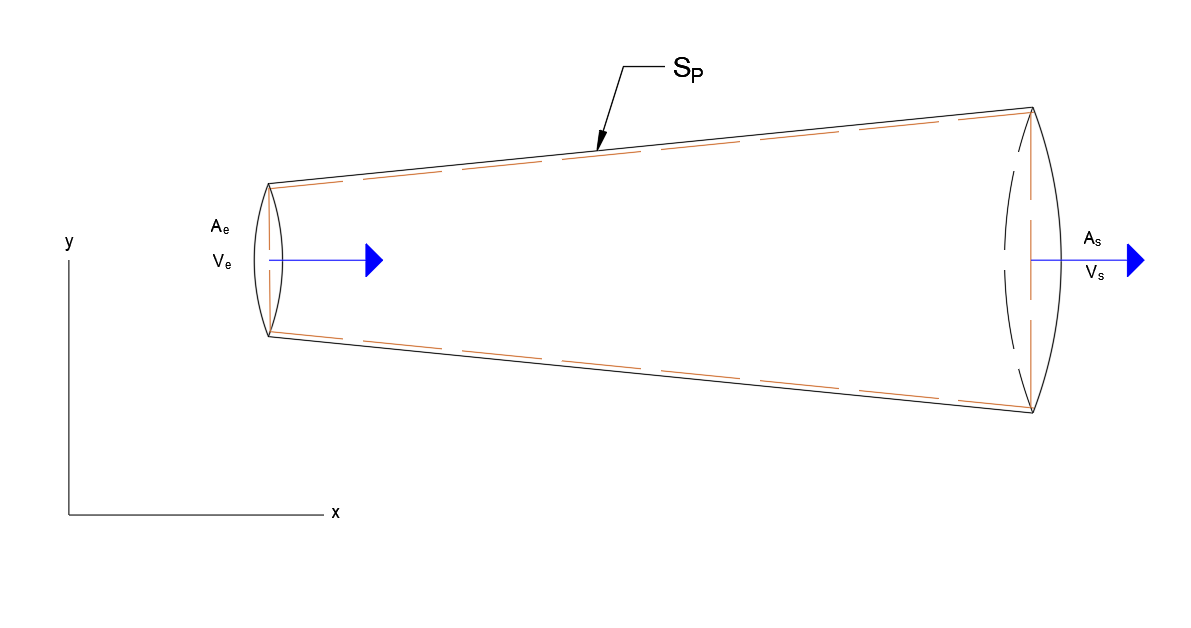
\includegraphics[width=0.7\linewidth]{imagenesEjercicios/tuberiaDivergente}
		\caption{Esquema de la tubería.}
		\label{fig:tuberiadivergente}

	\[\textcolor{blue}{\text{Se parte de la ecuación de conservación de la masa.}}\]
	\[\textcolor{blue}{\frac{d}{dt}\iiint_{V_c(t)}\rho\,dV+\oiint_{S_c(t)} \rho\left[(\vec{v}-\vec{v}_c)\cdot\vec{n}\right] \,dS=0}\]
\[\textcolor{blue}{
	\frac{d}{dt}\iiint_{V_c(t)}\rho\,dV=0 \rightarrow \text{El volumen no varia con el tiempo.}
}\]
\[\textcolor{blue}{
	\oiint_{S_c(t)} \rho\left[(\vec{v}-\vec{v}_c)\cdot\vec{n}\right] \,dS=
	\iint_{S_e(t)} \rho\left[(\vec{v}-\vec{v}_c)\cdot\vec{n}\right] \,dS+
	\iint_{S_p(t)} \rho\left[(\vec{v}-\vec{v}_c)\cdot\vec{n}\right] \,dS+
	\iint_{S_p(t)} \rho\left[(\vec{v}-\vec{v}_c)\cdot\vec{n}\right] \,dS
}\]
\[\textcolor{blue}{
	\iint_{S_e(t)} \rho\left[(\vec{v}-\vec{v}_c)\cdot\vec{n}\right] \,dS=-\rho v_e \iint_{S_e(t)}  \,dS=-\rho v_e A_e
}\]
\[\textcolor{blue}{
	\iint_{S_s(t)} \rho\left[(\vec{v}-\vec{v}_c)\cdot\vec{n}\right] \,dS=\rho v_s \iint_{S_s(t)}  \,dS=\rho v_s A_s
}\]
\textcolor{blue}{
	\[\iint_{S_p(t)} \rho\left[(\vec{v}-\vec{v}_c)\cdot\vec{n}\right] \,dS=0 \]
	 El volumen de control no se desplaza y el fluido  en contacto con las paredes tiene la misma velocidad que estas que al no moverse es 0.}

\textcolor{blue}{Por tanto:
\[-\rho v_e A_e+\rho v_s A_s=0\rightarrow v_e A_e=v_s A_s\]}
	\end{figure}
\newpage	
	\item Calcular la relación entre la velocidad de salida y la altura en un depósito con un agujero en su fondo
	\begin{figure}[H] 
		\centering
		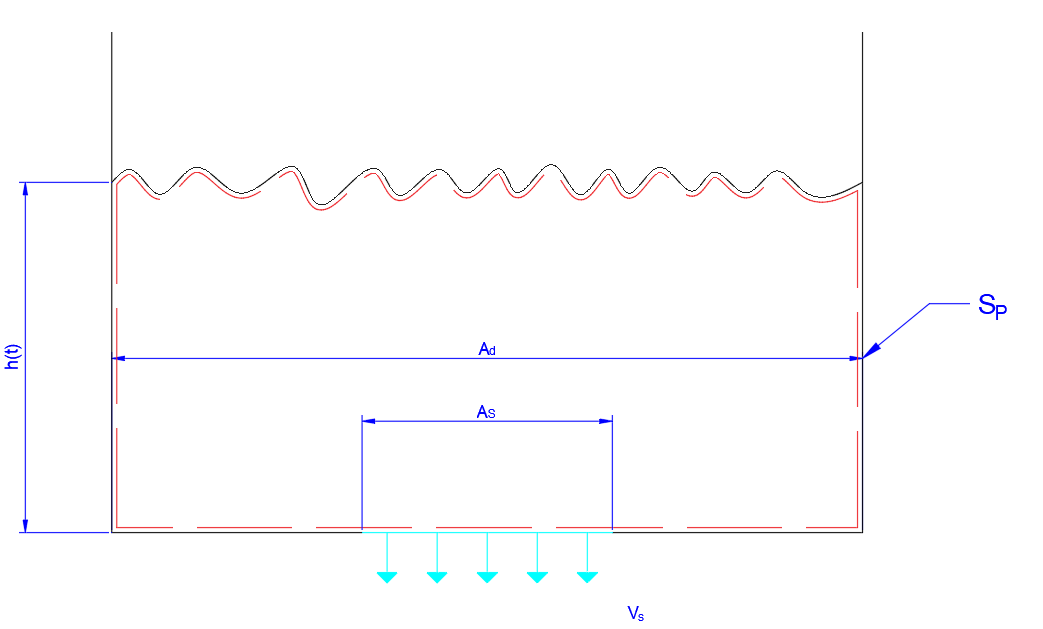
\includegraphics[width=0.7\linewidth]{imagenesEjercicios/depositoBujero}
		\caption{Esquema del depósito con el agujero en su fondo.}
		\label{fig:depositobujero}
	\[\textcolor{blue}{\text{Se parte de la ecuación de conservación de la masa.}}\]
\[\textcolor{blue}{\frac{d}{dt}\iiint_{V_c(t)}\rho\,dV+\oiint_{S_c(t)} \rho\left[(\vec{v}-\vec{v}_c)\cdot\vec{n}\right] \,dS=0}\]
\[\textcolor{blue}{
	\frac{d}{dt}\iiint_{V_c(t)}\rho\,dV=\rho \frac{d}{dt} V(t)=\rho A_d \dot{h}(t)
}\]
\[\textcolor{blue}{
	\oiint_{S_c(t)} \rho\left[(\vec{v}-\vec{v}_c)\cdot\vec{n}\right] \,dS=
	\iint_{S_s(t)} \rho\left[(\vec{v}-\vec{v}_c)\cdot\vec{n}\right] \,dS+
	\iint_{S_p(t)} \rho\left[(\vec{v}-\vec{v}_c)\cdot\vec{n}\right] \,dS+
	\iint_{S_n(t)} \rho\left[(\vec{v}-\vec{v}_c)\cdot\vec{n}\right] \,dS
}\]
\[\textcolor{blue}{
	\iint_{S_s(t)} \rho\left[(\vec{v}-\vec{v}_c)\cdot\vec{n}\right] \,dS=\rho v_s \iint_{S_s(t)}  \,dS=\rho v_s A_s
}\]
\[\textcolor{blue}{
	\iint_{S_n(t)} \rho\left[(\vec{v}-\vec{v}_c)\cdot\vec{n}\right] \,dS=0 \rightarrow \text{$v_c=v$ Y por tanto, se cancelan.}
}\]
\[\textcolor{blue}{
	\iint_{S_p(t)} \rho\left[(\vec{v}-\vec{v}_c)\cdot\vec{n}\right] \,dS=0
}\]
\textcolor{blue}{Por tanto:
	\[\rho A_d \dot{h}(t)+\rho v_s(t) A_s=0 \rightarrow A_d \dot{h}(t)+ v_s(t) A_s=0\]}
	\end{figure}
	
	\newpage
	\item Un envase que contiene aire comprimido se abre y el aire sale por el orificio con un gasto
	másico $\dot{m }$ = $C\rho$, donde $\rho$ es la densidad del aire del depósito y C es una constante. Se
	pide una expresión de la densidad en función del tiempo sabiendo que$\rho_0$ es la densidad
	inicial en el depósito y V su volumen, así como el tiempo necesario para que la densidad
	haya disminuido un 40 \%.
		\[\textcolor{blue}{\text{Se parte de la ecuación de conservación de la masa.}}\]
		\[\textcolor{blue}{\text{El volumen es constante y $\rho = f(t)$ con $\dot{m}=C\rho$}}\]
	\[\textcolor{blue}{\frac{d}{dt}\iiint_{V_c(t)}\rho\,dV+\oiint_{S_c(t)} \rho\left[(\vec{v}-\vec{v}_c)\cdot\vec{n}\right] \,dS=0}\]
	\[\textcolor{blue}{
		\frac{d}{dt}\iiint_{V_c(t)}\rho\,dV=V \frac{d}{dt} \rho(t)=V \dot{\rho}(t)
	}\]
	
	\textcolor{blue}{Como ya se ha hecho en los ejercicios anteriores, se descompone la superficie y como solo existe velocidad en el orificio:
	\[\oiint_{S_c(t)} \rho\left[(\vec{v}-\vec{v}_c)\cdot\vec{n}\right] \,dS=\rho v_s A_s = \dot{m}=C\rho\]	
	Por tanto:
	\[V \dot{\rho}(t)+C\rho(t)=0\]
	Que no es más que una EDO con variables separables cuya solución es:
	\[ln\left(\frac{\rho(t)}{\rho _0}\right)=-\frac{C}{V}t \rightarrow \text{Para una reducción de rho de un 40 \%} \rightarrow t=\frac{V}{C}ln\left(\frac{1}{0.6}\right)\]}
	\newpage
	\item Un tanque cilíndrico de diámetro (D) igual a 80 cm se comunica por el fondo con una
	tubería horizontal de diámetro (d) 15 cm por la que fluye agua. La
	velocidad del agua aguas arriba y aguas abajo del depósito es de 2,4 m/s y 1,8 m/s,
	respectivamente. En un instante de tiempo, la altura de agua (h) en el depósito es de 35
	cm. Calcular el tiempo que se necesita para rellenar el depósito que tiene una altura de
	1.2 m.
	\begin{figure}[H] 
		\centering
		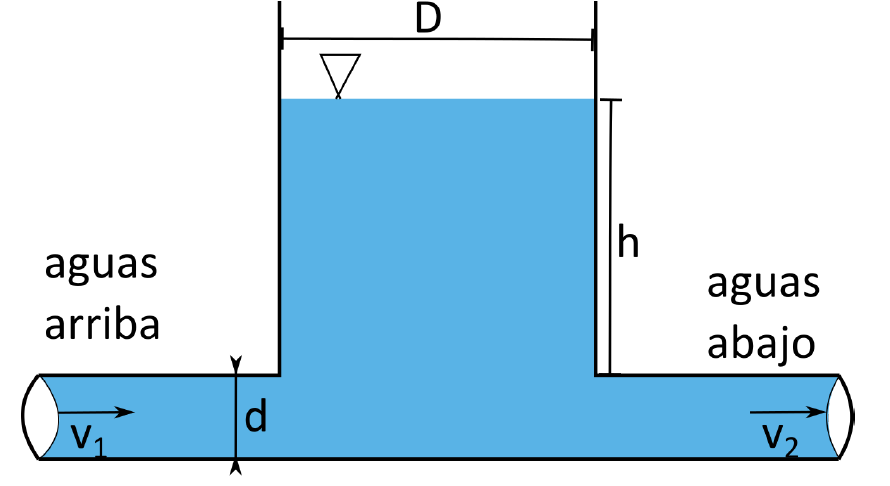
\includegraphics[width=0.7\linewidth]{imagenesEjercicios/tuberiaDeposito}
		\caption{Esquema de la tubería con el depósito.}
		\label{fig:tuberiadeposito}
	\end{figure}
	\textcolor{blue}{
	Se escoge como volumen de control el contorno del líquido, diferenciando entre 4 regiones:
	\begin{itemize}
		\item Entrada
		\item Salida
		\item Superficie depósito
		\item Pared
	\end{itemize}
	Partiendo de la ecuación de la masa y basandose en desarrollos anteriores:
	\[\frac{d}{dt}\iiint_{V_c(t)}\rho\,dV+\oiint_{S_c(t)} \rho\left[(\vec{v}-\vec{v}_c)\cdot\vec{n}\right] \,dS=0\]
	Como $\rho= cte$:
	\[\frac{d}{dt}\iiint_{V_c(t)}\,dV+\oiint_{S_c(t)} \left[(\vec{v}-\vec{v}_c)\cdot\vec{n}\right] \,dS=0\]
	\[\frac{d}{dt}\left[\pi \frac{D^2}{4}h(t)+l_{H}\pi\frac{d^2}{4}\right]-v_e\pi\frac{d^2}{4}+v_s\pi\frac{d^2}{4}=0\]
	\[D^2\dot{h}(t)-v_e d^2+v_s d^2=0\]
	Resolviendo la EDO
	\[h(t)=h_0+\frac{d^2}{D^2}\left(v_e-v_s\right) t\rightarrow \text{Sustituyendo los datos del enunciado se obtiene} \rightarrow t=40.3s\]
	}
	\item Se dispone de un émbolo de diámetro ($D_c$) con su superficie perforada con N agujeros de
	diámetro d que se disponen equidistantes al centro. Inicialmente el cilindro
	se encuentra lleno de un fluido incompresible de densidad $\rho$. El émbolo se desplaza con
	una velocidad $w_0$, produciéndose la salida del fluido con velocidad $v_s$ por un orificio de
	diámetro $D_s$. Se pide calcular la velocidad $v_s$ en función de los datos del ejercicio.
	\begin{figure}[H] 
		\centering
		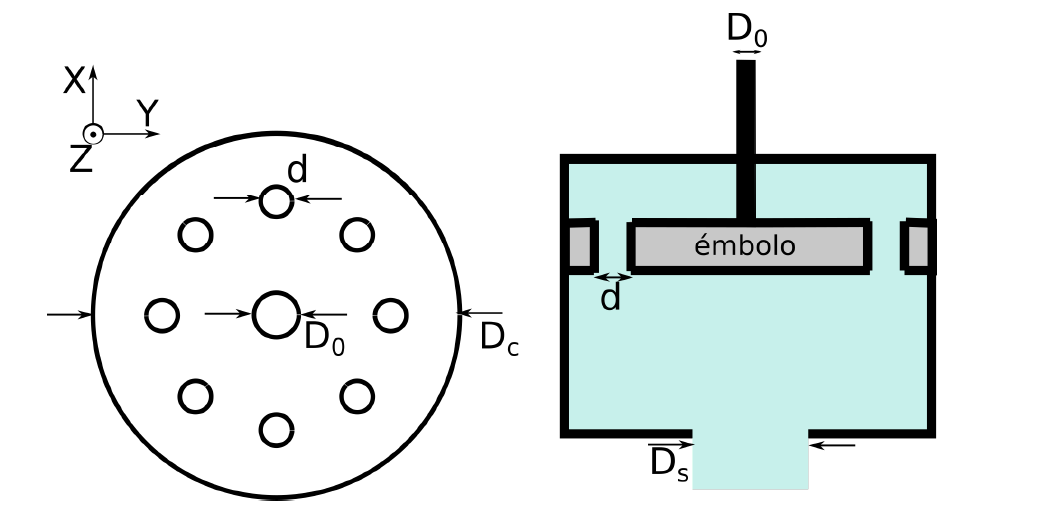
\includegraphics[width=0.7\linewidth]{imagenesEjercicios/emboloPerforado}
		\caption{Esquema del émbolo Perforado.}
		\label{fig:emboloperforado}

	\end{figure}
	\textcolor{blue}{
		Se escoge el volumen de control marcado sobre la figura y se plantea la ecuación de conservación de la masa:
	\[\frac{d}{dt}\iiint_{V_c(t)}\rho\,dV+\oiint_{S_c(t)} \rho\left[(\vec{v}-\vec{v}_c)\cdot\vec{n}\right] \,dS=0\]
	Como $\rho=cte$:
	\[\frac{d}{dt}\iiint_{V_c(t)}\,dV+\oiint_{S_c(t)} \left[(\vec{v}-\vec{v}_c)\cdot\vec{n}\right] \,dS=0\]
	El término local, como la única variación del volumen ocurre por la introducción de la varilla:
	\[\frac{d}{dt}\iiint_{V_c(t)}\,dV=-\omega _0 \pi \frac{D^2_0}{4}\]
	El término convectivo, teniendo en cuenta que las superficies son la pared o la de salida:
	\[\oiint_{S_c(t)} \left[(\vec{v}-\vec{v}_c)\cdot\vec{n}\right] \,dS=v_s \pi \frac{D^2_s}{4}\]
	Por tanto:
	\[-\omega _0 \pi \frac{D^2_0}{4}+v_s \pi \frac{D^2_s}{4}=0\rightarrow v_s=\omega _0 \left(\frac{D_0}{D_s}\right)^2\]
	}	
	
	\newpage
	\item Calcular en función de la altura la relación con la velocidad de un depósito con varios agujeros
	\begin{figure}[H]
		\centering
		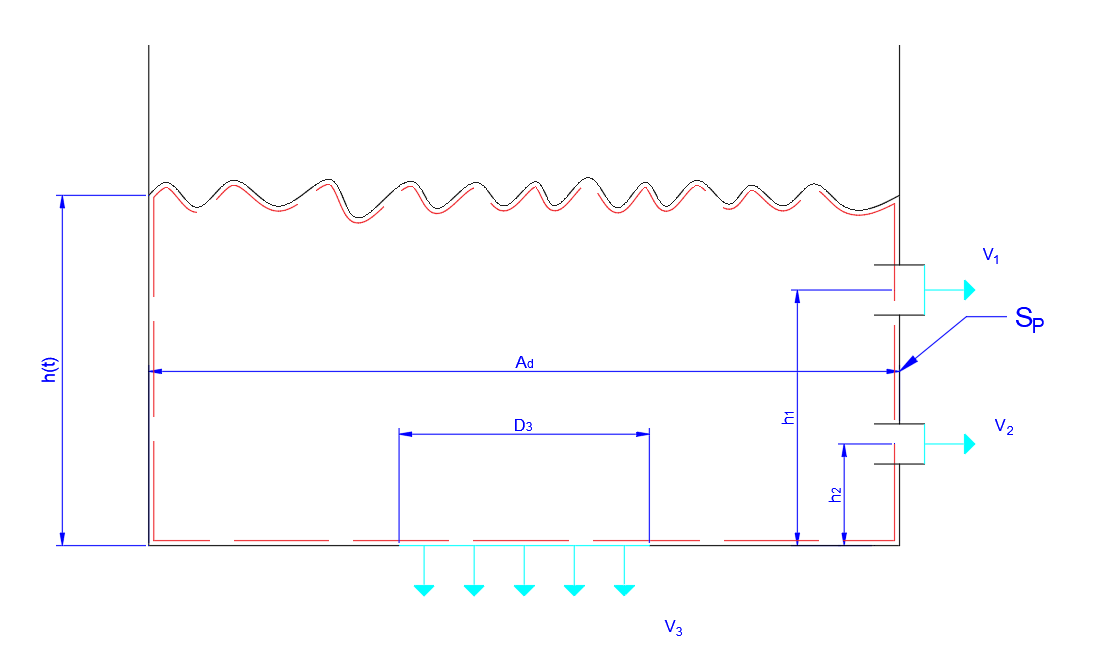
\includegraphics[width=0.7\linewidth]{imagenesEjercicios/depositoVariosBujeros}
		\caption{Esquema del depósito con varios agujeros.}
		\label{fig:depositovariosbujeros}
	\end{figure}
\textcolor{blue}{
Teniendo en cuenta los resultados obtenidos anteriormente para un depósito, se pueden plantear directamente las ecuaciones teniendo en cuenta las distintas regiones:
\begin{itemize}
	\item $h(t)>h_1$
	\[-A_d\dot{h}(t)=v_3\frac{\pi D^2_3}{4}+v_2\frac{\pi D^2_2}{4}+v_1\frac{\pi D^2_1}{4}\]
	\item $h_1>h(t)>h_2$
	\[-A_d\dot{h}(t)=v_3\frac{\pi D^2_3}{4}+v_2\frac{\pi D^2_2}{4}\]
	\item $h(t)<h_2$
	\[-A_d\dot{h}(t)=v_3\frac{\pi D^2_3}{4}\]
\end{itemize}
}

	\newpage
	\item El flujo de un fluido está representado por el siguiente campo de velocidades: u = u (x, t);
	v = 0; w = 0, y densidad $\rho$ =  $\rho _0$ [a - cos ($\omega$t)] con a$>$1. Determinar la función v (x, t)
	sabiendo que v (0, t) = $v_0$.
	\textcolor{blue}{
	\[\rho =  \rho _0 [a - cos (\omega t)] \ y \ v=f(x,t)\]
	Se plantea la ecuación de conservación de la masa en forma diferencial:
	\[\frac{\partial \rho}{\partial t} +\vec{\nabla}\cdot\left(\rho\vec{v}\right)=0\]
	\[\frac{\partial}{\partial t}\left(\rho _0 [a - cos (\omega t)]\right)+\left[\frac{\partial}{\partial x}\vec{i}+
	\frac{\partial}{\partial y}\vec{j}+
	\frac{\partial}{\partial z}\vec{k}\right]\cdot \left[ \rho _0 [a - cos (\omega t)] \right]v(x,t)=0\]
	\[
	\omega \rho _0 sen(\omega t)+\left[ \rho _0 [a - cos (\omega t)] \right]\frac{\partial}{\partial x}v(x,t)=0
	\]
	\[\frac{\partial}{\partial x}v(x,t)=-\frac{\omega sen(\omega t)}{a - cos (\omega t)}\]
	Resolviendo la EDO con la condición de que v (0, t) = $v_0$.
	\[v(x,t)=-\frac{\omega sen(\omega t)}{a - cos (\omega t)}x+v_0\]
	}
\end{enumerate}
\newpage
\subsection{Tema 4: Conservación de la cantidad de movimiento}
\begin{enumerate}
	\item Considérese una tubería de sección decreciente con un codo con un ángulo $\alpha$. Calcule la fuerza que se ejerce sobre las paredes.
	\begin{figure}[H]
		\centering
		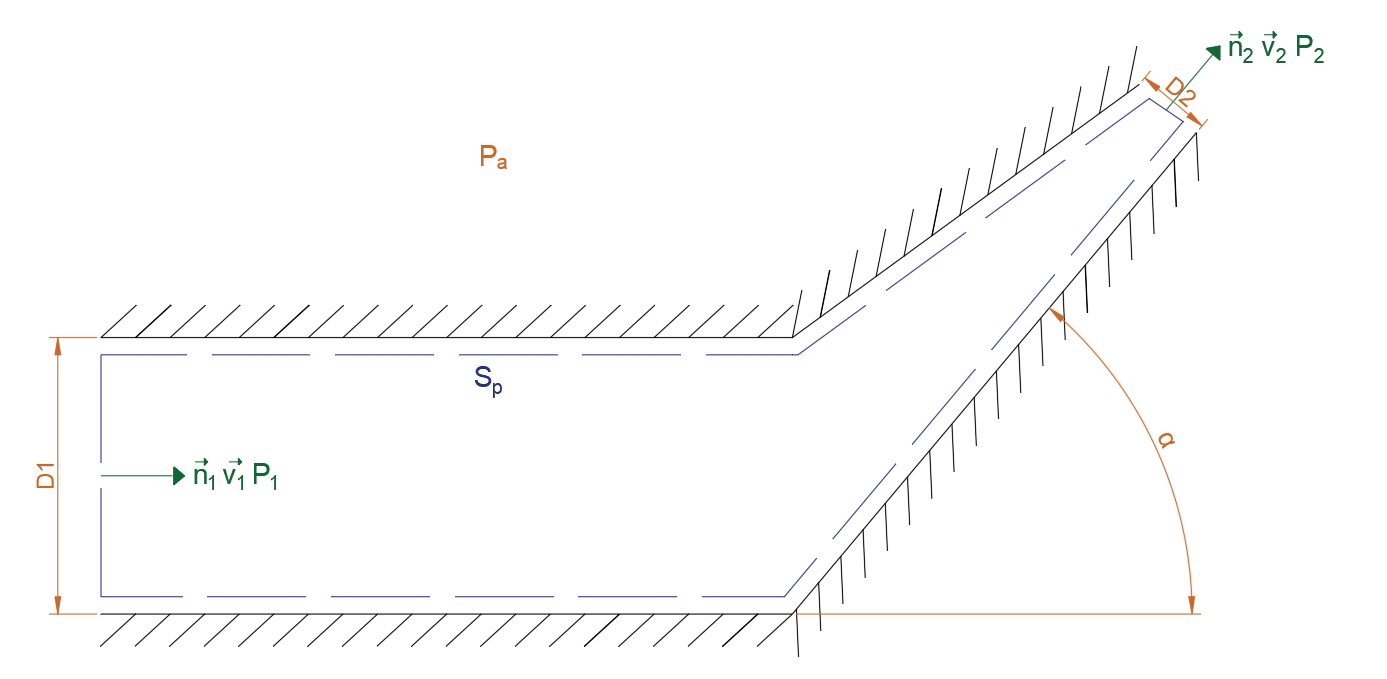
\includegraphics[width=0.7\linewidth]{imagenesEjercicios/tuberiaCodoDecreciente}
		\caption{Esquema de la tubería.}
		\label{fig:tuberiacododecreciente}
	\end{figure}
	\textcolor{blue}{
	Se plantea la ecuación de conservación de la masa:  
	\[\frac{d}{dt}\iiint_{V_c}\rho\,dV+\oiint_{S_c} \rho\left[(\vec{v}-\vec{v}_c)\cdot\vec{n}\right] \,dS=0\]
	Como el fluido es globalmente estacionario y no varia el volumen:
	\[\rho\oiint_{S_c} \left[(\vec{v}-\vec{v}_c)\cdot\vec{n}\right] \,dS=0\]
	\[\oiint_{S_c} \left[(\vec{v}-\vec{v}_c)\cdot\vec{n}\right] \,dS=
	\iint_{S_1} \left[(\vec{v}-\vec{v}_c)\cdot\vec{n}\right] \,dS
	+
	\iint_{S_2} \left[(\vec{v}-\vec{v}_c)\cdot\vec{n}\right] \,dS
	+
	\iint_{S_p} \left[(\vec{v}-\vec{v}_c)\cdot\vec{n}\right] \,dS\]
	\[\iint_{S_1} \left[(\vec{v}-\vec{v}_c)\cdot\vec{n}\right] \,dS=-v_1\pi\frac{D_1^2}{4}\]
	\[\iint_{S_2} \left[(\vec{v}-\vec{v}_c)\cdot\vec{n}\right] \,dS=v_2\pi\frac{D_2^2}{4}\]
	\[\iint_{S_p} \left[(\vec{v}-\vec{v}_c)\cdot\vec{n}\right] \,dS=0\]
	Por tanto de la conservación de la masa se obtiene:
	\[v_1D_1^2=v_2D_2^2\]
	Planteando la conservación de la cantidad de movimiento
	\[\iiint_{V_c}\vec{f}_V\,dV
	+
	\oiint_{S_c}\left(-P\overline{\overline{I}}+\overline{\overline{\tau}}\right)\cdot\vec{n}\,dS=
	\iiint_{V_c}\frac{\partial \rho\vec{v}}{\partial t}\,dV
	+\oiint_{S_c}\rho\vec{v}\left[\left(\vec{v}-\vec{v}_c\right)\cdot\vec{n}\right]\,dS\]
	El término de fuerzas volumétricas:
	\[\iiint_{V_c}\vec{f}_V\,dV=\iiint_{V_f}\rho\vec{g}\,dV=\rho \vec{g}V_c\]
	El término de fuerzas superficiales:
	\[\oiint_{S_c}\left(-P\overline{\overline{I}}+\overline{\overline{\tau}}\right)\cdot\vec{n}\,dS=
	\iint_{S_1}\left(-P\overline{\overline{I}}+\overline{\overline{\tau}}\right)\cdot\vec{n}\,dS
	+
	\iint_{S_2}\left(-P\overline{\overline{I}}+\overline{\overline{\tau}}\right)\cdot\vec{n}\,dS
	+
	\iint_{S_p}\left(-P\overline{\overline{I}}+\overline{\overline{\tau}}\right)\cdot\vec{n}\,dS
	\]
	\begin{itemize}
		\item 	Como se cumple que la fuerza ejercida por la atmósfera sobre toda la superficie de control es nula:
		\[\oiint_{S_c}P_a\vec{n}\,dS=0\]
		\item Por tanto, para tener en cuenta las aportaciones de fuerza tanto del fluido como de la presión atmosférica:
		\[\oiint_{S_c}\left(-P\overline{\overline{I}}+\overline{\overline{\tau}}\right)\cdot\vec{n}\,dS=\oiint_{S_c}\left[-(P-P_a)\overline{\overline{I}}+\overline{\overline{\tau}}\right]\cdot\vec{n}\,dS\]
		\item Además, el término de fuerza superficial sobre las paredes es la fuerza a calcular:
		\[\iint_{S_p}\left[-(P-P_a)\overline{\overline{I}}+\overline{\overline{\tau}}\right]\cdot\vec{n}\,dS=-F_{fluido+atm\rightarrow pared}\]
		\item En un perfil uniforme se cumple que $\tau_v$ es despreciable frente al término de presión. Por tanto:
		\[\oiint_{S_c}\left(-P\overline{\overline{I}}+\overline{\overline{\tau}}\right)\cdot\vec{n}\,dS=
		\iint_{S_1}-(P-P_a)\vec{n}\,dS
		+
		\iint_{S_2}-(P-P_a)\vec{n}\,dS
		-F_{fluido\rightarrow pared}\]
		\[\oiint_{S_c}\left(-P\overline{\overline{I}}+\overline{\overline{\tau}}\right)\cdot\vec{n}\,dS=
		-(P_1-P_a)\frac{\pi D^2_1}{4}(-\vec{i})
		-(P_2-P_a)\frac{\pi D^2_2}{4}(\vec{n})
		-F_{fluido+atm\rightarrow pared}\]
		\[\oiint_{S_c}\left(-P\overline{\overline{I}}+\overline{\overline{\tau}}\right)\cdot\vec{n}\,dS=
		\frac{\pi}{4}\left[(P_1-P_a) D^2_1\vec{i}-(P_2-P_a)D^2_2\left(cos(\alpha)\vec{i}+sen(\alpha)\vec{j}\right)\right]
		-F_{fluido+atm\rightarrow pared}\]
	\end{itemize}
	El término local:
	\[\iiint_{V_c}\frac{\partial \rho\vec{v}}{\partial t}\,dV=0\]
	El término convectivo:
	\[\oiint_{S_c}\rho\vec{v}\left[\left(\vec{v}-\vec{v}_c\right)\cdot\vec{n}\right]\,dS=
	\iint_{S_1}\rho\vec{v}\left[\left(\vec{v}-\vec{v}_c\right)\cdot\vec{n}\right]\,dS+
	\iint_{S_2}\rho\vec{v}\left[\left(\vec{v}-\vec{v}_c\right)\cdot\vec{n}\right]\,dS
	+\iint_{S_p}\rho\vec{v}\left[\left(\vec{v}-\vec{v}_c\right)\cdot\vec{n}\right]\,dS\]
	\[\iint_{S_1}\rho\vec{v}\left[\left(\vec{v}-\vec{v}_c\right)\cdot\vec{n}\right]\,dS=\rho v_1\vec{i}\cdot v_1\vec{i}\cdot-\vec{i}\frac{D^2_1}{\pi}=-\rho v^2_1\frac{D^2_1}{\pi}\vec{i}\]
	\[\iint_{S_2}\rho\vec{v}\left[\left(\vec{v}-\vec{v}_c\right)\cdot\vec{n}\right]\,dS=\rho v_2\vec{n}\cdot v_2\vec{n}\cdot\vec{n}\frac{D^2_2}{\pi}=\rho v^2_2\frac{D^2_2}{\pi}\vec{n}=\rho v^2_2\frac{D^2_2}{\pi}\left[cos(\alpha)\vec{i}+sen(\alpha)\vec{j}\right]\]
	\[\iint_{S_p}\rho\vec{v}\left[\left(\vec{v}-\vec{v}_c\right)\cdot\vec{n}\right]\,dS=0\]
	Por tanto, sustituyendo los término se obtiene:
	\[F_{fluido+atm\rightarrow pared}=\frac{\pi}{4}\left[(P_1-P_a) D^2_1\vec{i}-(P_2-P_a)D^2_2\vec{n}\right]+\rho g V_c \vec{j}
	+\rho\frac{\pi}{4}\left[v^2_1D^2_1\vec{i}-v^2_2D^2_2\vec{n}\right] \]
	\[\vec{n}=cos(\alpha)\vec{i}+sen(\alpha)\vec{j}\]
	}
		
	
	
	
	
	\item Se tiene un elemento de área de 2 $mm^2$ cuya normal es paralela al vector de componentes
	(1, 2, 3). Si el tensor de esfuerzos es de la forma $\tau_{xx} = -2 \times 10^5; \tau_{yy} = -110 \times 10^ 3; \tau_{zz} =
	-115 \times 10^3; \tau_{xy} = 1\times10^3; \tau_{xz} = -5 \times 10^4;  \tau_{zy} = 1 \times 10^5$, todos ellos en pascales. Se pide:
	\begin{itemize}
		\item 	El tensor de esfuerzos
		\textcolor{blue}{
		\[\overline{\overline{\tau}}=\begin{bmatrix}
			\tau_{xx} &\tau_{xy}&\tau_{xz}\\
				\tau_{yx} &\tau_{yy}&\tau_{yz}\\
					\tau_{zx} &\tau_{zy}&\tau_{zz}\\
		\end{bmatrix}=
		\begin{bmatrix}
		 -2 \times 10^5&1\times10^3&-5 \times 10^4\\
		1\times10^3& -110 \times 10^ 3&1 \times 10^5\\
		 -5 \times 10^4&1 \times 10^5&-115 \times 10^3\\
		\end{bmatrix}
		\]}
		\item El valor de la fuerza superficial sobre dicha área  si la presión es de 1.5 bares.
			\textcolor{blue}{\[F=\oiint_{S_c}\left(-p\overline{\overline{I}}+\overline{\overline{\tau}}\right)\cdot\vec{n}\,dS=\left(-p\overline{\overline{I}}+\overline{\overline{\tau}}\right)\cdot\vec{n}S \]
			\[	F=-1.5\times10^5 \frac{2\times 10^{-6}}{\sqrt{1^2+2^2+3^2}}\begin{bmatrix}
					1 \\
					2 \\
					3 \\
				\end{bmatrix}+	\begin{bmatrix}
				-2 \times 10^5&1\times10^3&-5 \times 10^4\\
				1\times10^3& -110 \times 10^ 3&1 \times 10^5\\
				-5 \times 10^4&1 \times 10^5&-115 \times 10^3\\
				\end{bmatrix}\cdot\frac{2\times 10^{-6}}{\sqrt{1^2+2^2+3^2}}\begin{bmatrix}
				1 \\
				2 \\
				3 \\
				\end{bmatrix}\]
			\[F=\frac{1}{\sqrt{14}}\begin{bmatrix}
				-0.996 \\
				-0.438 \\
				-1.29 \\
			\end{bmatrix}\]}
	\end{itemize}
\newpage
	

	\item Considérese un depósito cilíndrico de sección A que se encuentra fijo sobre una plataforma. El depósito tiene una altura h de agua y en el instante inicial se practica
	un orificio de área $A_s$ en la parte inferior de la pared. ¿Hacia dónde tendería a desplazarse
	si no estuviera fijado a la plataforma? Calcular la fuerza de reacción de la plataforma sobre
	el depósito.
 \begin{figure}[H]
 	\centering
 	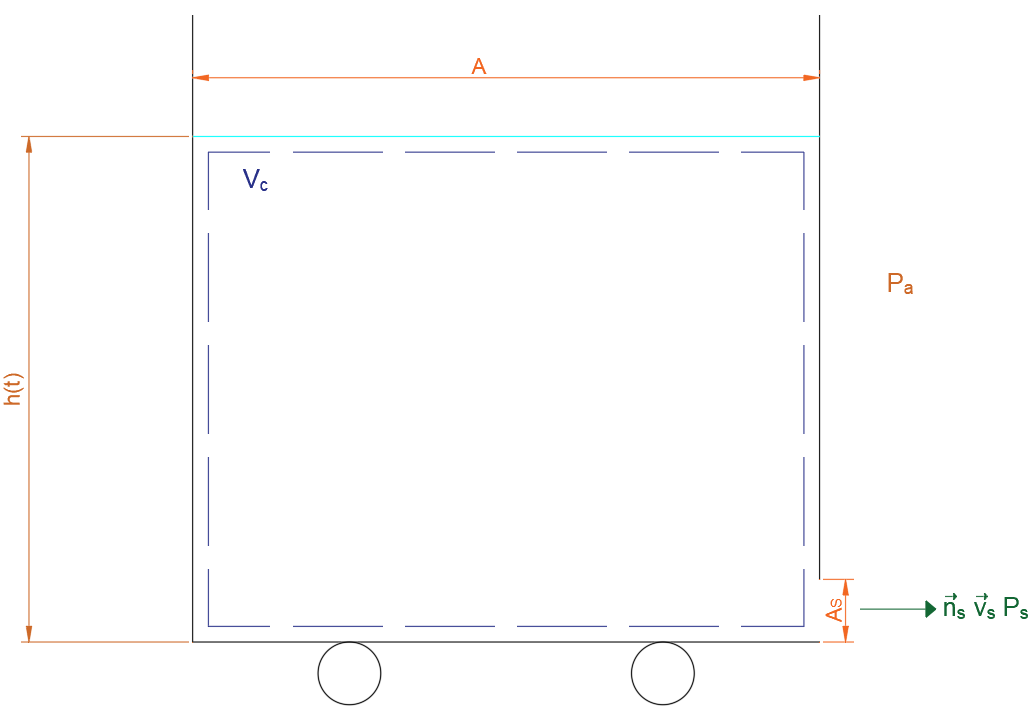
\includegraphics[width=0.7\linewidth]{imagenesEjercicios/depositobloqueado}
 	\caption{Esquema del depósito.}
 	\label{fig:depositobloqueado}
 \end{figure}
 \textcolor{blue}
 {
 	Se plantea la ecuación de conservación de la masa: 
 	\[\frac{d}{dt}\iiint_{V_c}\rho\,dV+\oiint_{S_c} \rho\left[(\vec{v}-\vec{v}_c)\cdot\vec{n}\right] \,dS=0\]
 	Teniendo en cuenta desarrollos de ejercicios anteriores:
 	\[A\dot{h}(t)=v_s(t)A_s\]
 	Planteando la conservación de la cantidad de movimiento, donde solo se buscan los términos en dirección $\vec{i}$ ya que el depósito si no estuviese fijo se movería hacia la izquierda y los términos de fuerza en dirección al suelo solo soportan el peso del depósito y no intervendrían en este ''movimiento''
 	\[\iiint_{V_c}\vec{f}_V\,dV
 	+
 	\oiint_{S_c}\left(-P\overline{\overline{I}}+\overline{\overline{\tau}}\right)\cdot\vec{n}\,dS=
 	\iiint_{V_c}\frac{\partial \rho\vec{v}}{\partial t}\,dV
 	+\oiint_{S_c}\rho\vec{v}\left[\left(\vec{v}-\vec{v}_c\right)\cdot\vec{n}\right]\,dS\]
 	El término de fuerzas volumétricas es nulo en la dirección de la fuerza a reacción a calcular:
 	\[\iiint_{V_c}\vec{f}_V\,dV=0\]
 	El término de fuerzas superficiales:
 	\[\oiint_{S_c}\left(-P\overline{\overline{I}}+\overline{\overline{\tau}}\right)\cdot\vec{n}\,dS=
 	\iint_{S_s}\left(-P\overline{\overline{I}}+\overline{\overline{\tau}}\right)\cdot\vec{n}\,dS
 	+
 	\iint_{S_n}\left(-P\overline{\overline{I}}+\overline{\overline{\tau}}\right)\cdot\vec{n}\,dS
 	+
 	\iint_{S_p}\left(-P\overline{\overline{I}}+\overline{\overline{\tau}}\right)\cdot\vec{n}\,dS
 	\]
 	\begin{itemize}
 		\item En un perfil uniforme se cumple que $\tau_v$ es despreciable frente al término de presión. Por tanto la resultante en la dirección $\vec{i}$:
 		\[\oiint_{S_c}\left(-P\overline{\overline{I}}+\overline{\overline{\tau}}\right)\cdot\vec{n}\,dS\cdot\vec{i}=
 		\left[
 		\iint_{S_s}-(P-P_a)\vec{n}\,dS
 		+
 		\iint_{S_n}-(P-P_a)\vec{n}\,dS
 		+
 		\iint_{S_p}-(P-P_a)\vec{n}\,dS
 		\right]\cdot\vec{i}
 		\]
 		\[\oiint_{S_c}\left(-P\overline{\overline{I}}+\overline{\overline{\tau}}\right)\cdot\vec{n}\,dS\cdot\vec{i}=
 		(P_s-P_a)A_s
 		+0
 		-F_{fl+atm\rightarrow dep}=(P_s-P_a)A_s -F_{fl+atm\rightarrow dep}\]
 	\end{itemize}
 	El término local es nulo debido a que la variación de la derivada de la altura tiene un orden de magnitud mucho menor al resto de términos y, por tanto es despreciable :
 	\[\iiint_{V_c}\frac{\partial \rho\vec{v}}{\partial t}\,dV=0\]
 	El término convectivo en la dirección de $\vec{i}$:
 	\[\oiint_{S_c}\rho\vec{v}\left[\left(\vec{v}-\vec{v}_c\right)\cdot\vec{n}\right]\,dS=
 	\iint_{S_n}\rho\vec{v}\left[\left(\vec{v}-\vec{v}_c\right)\cdot\vec{n}\right]\,dS+
 	\iint_{S_s}\rho\vec{v}\left[\left(\vec{v}-\vec{v}_c\right)\cdot\vec{n}\right]\,dS
 	+\iint_{S_p}\rho\vec{v}\left[\left(\vec{v}-\vec{v}_c\right)\cdot\vec{n}\right]\,dS\]
 	\[\oiint_{S_c}\rho\vec{v}\left[\left(\vec{v}-\vec{v}_c\right)\cdot\vec{n}\right]\,dS\cdot\vec{i}=
 	0+
 	\rho v^2_s A_s \vec{i}\cdot\vec{i}
 	+0=	\rho v^2_s A_s\]
 	Por tanto, sustituyendo los término se obtiene:
	 \[(P_s-P_a)A_s -F_{fl+atm\rightarrow dep}=\rho v^2_s A_s\rightarrow P_s=P_a\]
	 \[|F_{fl+atm\rightarrow dep}|=|\rho v^2_s A_s|\rightarrow  \text{Como se mueve a la izquierda: } \vec{F}_{fl+atm\rightarrow dep}= -\rho v^2_s A_s\vec{i}\]
	 Para obtener la relación entre altura y velocidad de salida se aplica el teorema de Bernouilli entre la parte superior del depósito y la salida:
	 \[P_1+\rho g h(t)=P_s+\frac{v^2_s(t)}{2}\rho\rightarrow P_1=P_s=P_a \rightarrow h(t)=\frac{v^2_s(t)}{2g}\rightarrow v_s(t)=\sqrt{2gh(t)}\]
	 Aplicando esta expresión junto a la obtenida con la conservación de la masa:
	 \[v_s(t)=\sqrt{2gh(t)}\]
	 \[A\dot{h}(t)=v_s(t)A_s\]
	 Resolviendo la EDO se obtiene:
	 \[\sqrt{h(t)}=\frac{-A_s}{A}\sqrt{\frac{g}{2}}t+\sqrt{h_0}\]
}
%\item Considérese el siguiente chorro impactando contra una placa de forma axilsimétrica.
%
%\begin{figure}[H]
%	\centering
%		\begin{circuitikz}
%			\tikzstyle{every node}=[font=\large]
%			\draw  (-5.5,15.75) rectangle (-3.25,15.25);
%			\draw  (-5.5,13.25) rectangle (-3.25,12.75);
%			\draw [ color={rgb,255:red,0; green,128; blue,255}, short] (-3.25,15.25) -- (0,15.25);
%			\draw [ color={rgb,255:red,0; green,128; blue,255}, short] (0,15.25) .. controls (1,15.25) and (1.25,15.5) .. (1.25,16.5);
%			\draw [ color={rgb,255:red,0; green,128; blue,255}, short] (1.25,16.5) -- (1.25,18.5);
%			\draw [ color={rgb,255:red,0; green,128; blue,255}, short] (-3.25,13.25) -- (0,13.25);
%			\draw [ color={rgb,255:red,0; green,128; blue,255}, short] (0,13.25) .. controls (1.25,13.25) and (1.25,13) .. (1.25,12);
%			\draw [ color={rgb,255:red,0; green,128; blue,255}, short] (1.25,12) -- (1.25,10);
%			\draw [short] (1.5,18.5) -- (1.5,10);
%			\draw [short] (2.5,18.5) -- (2.5,10);
%			\draw [ color={rgb,255:red,0; green,128; blue,0}, -latex] (2,14.25) -- (2,15.75)node[pos=1,above]{$\vec{e}_r$};
%			\draw [-latex] (2,14.25) -- (4.5,14.25)node[pos=1,right]{$\vec{v}_p$};
%			\draw [ color={rgb,255:red,0; green,128; blue,0}, -latex] (2,14.25) -- (3.25,14.25)node[pos=1,above]{$\vec{k}$};
%			\draw [short] (-6,14.25) -- (-5,14.25);
%			\draw [short] (-4.75,14.25) -- (-4.5,14.25);
%			\draw [short] (-4.25,14.25) -- (-3.25,14.25);
%			\draw [short] (-3,14.25) -- (-2.75,14.25);
%			\draw [short] (-2.5,14.25) -- (-1.5,14.25);
%			\draw [short] (-1.25,14.25) -- (-1,14.25);
%			\draw [short] (-0.75,14.25) -- (0.25,14.25);
%			\draw [short] (0.5,14.25) -- (0.75,14.25);
%			\draw [short] (1,14.25) -- (2,14.25);
%			\draw [ color={rgb,255:red,255; green,0; blue,0}, -latex] (-5.5,14.75) -- (-3.5,14.75)node[pos=1,right]{$\vec{v}_e$};
%			\node [font=\large, color={rgb,255:red,0; green,128; blue,255}] at (-1.75,13.75) {$\rho=cte$};
%			\node [font=\large] at (-4.25,17.75) {$P_a$};
%			\draw [-latex] (0.75,17.75) -- (1.25,17.75)node[pos=0,above]{h(r)};
%			\draw [-latex] (2,17.75) -- (1.5,17.75);
%			\node [font=\large] at (1,15.25) {\textbf{r}};
%			\draw [-latex] (-5.5,9.75) -- (-4.25,9.75)node[pos=1,right]{$\vec{i}$};
%			\draw [-latex] (-5.5,9.75) -- (-5.5,11)node[pos=1,above]{$\vec{j}$};
%			\draw [ color={rgb,255:red,128; green,0; blue,255}, -latex] (1.25,11.75) -- (2.25,11.75)node[pos=0.5,above]{$\vec{n}_p$};
%			\draw [ color={rgb,255:red,128; green,0; blue,255}, -latex] (1,15.5) -- (0.25,16.25)node[pos=1,above]{$\vec{n}_{int}$};
%			\draw [ color={rgb,255:red,128; green,0; blue,255}, -latex] (-4.5,13.75) -- (-5.75,13.75)node[pos=0.4,above]{$\vec{n}_e$};
%			\draw [ color={rgb,255:red,128; green,0; blue,255}, -latex] (1.5,11.25) -- (1.5,10.25)node[pos=0.5,left]{$\vec{n}_r,$ $\vec{v}_r$};
%			\draw [ color={rgb,255:red,0; green,128; blue,255}, dashed] (-4.5,15.25) -- (-4.5,13.25);
%			\node [font=\large, color={rgb,255:red,0; green,128; blue,255}] at (0.25,13.75) {$V_C$};
%			\node [font=\large] at (-4.5,16) {Boquilla};
%			\node [font=\large] at (3.5,13.25) {$v_e>v_p$};
%			\draw [latex-latex] (-6,15.25) -- (-6,13.25)node[pos=0.5,left]{$D_e$};
%		\end{circuitikz}
%		
%		\begin{circuitikz}
%			\draw  (11,14.25) ellipse (2cm and 3cm);
%			\draw [short] (11,17.25) -- (9.75,17.25);
%			\draw [short] (11,11.25) -- (9.75,11.25);
%			\draw [short] (9.75,11.25) .. controls (8,12.25) and (7.75,16.25) .. (9.75,17.25);
%			\draw [-latex] (11,14.25) -- (11,17.25)node[pos=0.5,left]{r};
%			\draw [ color={rgb,255:red,0; green,128; blue,0}, -latex] (11,14.25) -- (10.5,15)node[pos=0.5,left]{$\vec{e}_r$};
%			\draw [latex-latex] (9.75,17.75) -- (11,17.75)node[pos=0.5,above]{h(r)};
%			\draw [ color={rgb,255:red,0; green,128; blue,255}, -latex] (9,15.75) -- (8.25,16)node[pos=1,above]{$\vec{e}_r,$ $\vec{v}_r$};
%		\end{circuitikz}
%	\caption{Esquema del chorro axilsimétrico.}
%	\label{fig:chorroaxil}
%\end{figure}
%
%Calcular la fuerza que ejerce el chorro junto con la presión atmosférica sobre la placa.
%
%\textcolor{blue}
%{
%	\textit{Conservación de la masa en forma integral:}
%	\[\dfrac{d}{dt} \iiint_{V_C}\rho dV + \oiint_{S_C} \rho (\vec{v}-\vec{v}_C)\cdot \vec{n} dS = 0\]
%	Asumiendo el sistema como globalmente estacionario:
%	\[\dfrac{d}{dt} \iiint_{V_C} \rho dV = 0; S_C = S_e \cup S_p \cup S_{int} \cup S_r\]
%	\[
%	\red
%	{
%		\underbrace
%		{
%			\blue \iint_{S_e}\rho (\vec{v}-\vec{v}_C)\cdot \vec{n}_e dS
%		}
%		_
%		{
%			\begin{matrix}
%				\vec{v}_C=\vec{0}\\
%				\vec{v}=-(v_e-v_p)\vec{k}\\
%				\vec{n}_e=-\vec{k}
%			\end{matrix}
%		}
%	}
%	\blue +
%	\red
%	{
%		\underbrace
%		{
%			\blue \iint_{S_p}\rho (\vec{v}-\vec{v}_C)\cdot \vec{n}_p dS
%		}
%		_
%		{
%			\begin{matrix}
%				\vec{v}_C=\vec{0}\\
%				\vec{v}=0\\
%				\vec{n}_p=\text{no importa}
%			\end{matrix}
%		}
%	}
%	\blue +
%	\red
%	{
%		\underbrace
%		{
%			\blue \iint_{S_{int}}\rho (\vec{v}-\vec{v}_C)\cdot \vec{n}_{int} dS
%		}
%		_
%		{
%			\begin{matrix}
%				\vec{v}_C=\vec{0}\\
%				\vec{v}=\vec{v}_{int}\\
%				\vec{n}_{int}\perp \vec{v}_{int}
%			\end{matrix}
%		}
%	}
%	\blue +
%	\red
%	{
%		\underbrace
%		{
%			\blue \iint_{S_{r}}\rho (\vec{v}-\vec{v}_C)\cdot \vec{n}_{r} dS
%		}
%		_
%		{
%			\begin{matrix}
%				\vec{v}_C=\vec{0}\\
%				\vec{v}=\vec{v}_{r} \cdot \vec{e}_r\\
%			\end{matrix}
%		}
%	}
%	\blue \Rightarrow
%	\]	
%	Sabiendo que $\vec{e}_r$ es un campo vectorial central y, por tanto \[\iint_S\vec{e}_rdS=0\Rightarrow\]
%	\[(v_e-v_p)\dfrac{\pi D_e^2}{4}=v_r2\pi rh(r)\]
%	\textit{Conservación de la cantidad de movimiento en forma integral:}
%	\[\dfrac{d}{dt} \iiint_{V_C}\rho \vec{v} dV + \oiint_{S_C} \rho \vec{v} (\vec{v}-\vec{v}_C)\cdot \vec{n} dS = \oiint_{S_C}(-p\cdot \bar{\bar{I}}+\bar{\bar{\tau}}_v)\cdot \vec{n}dS+\iiint_{V_C}\rho \vec{g} dV=(*)\]
%	\[\iiint_{V_C}\rho \vec{g} dV = 0\text{ al ser el número de Froude } Fr\uparrow\uparrow \]
%	\[\iint_{S_e\cup S_{int}\cup S_r} (-(p-p_a)\bar{\bar{I}} + \bar{\bar{\tau}}_v)\cdot \vec{n} dS = 0 \text{ al ser } P = P_a, \text{ flujo ideal uniforme } (Re\uparrow\uparrow) \Rightarrow \bar{\bar{\tau}}_v = \bar{\bar{0}}\]
%	\[(*)=-\rho(v_e-v_p)^2\cdot\dfrac{\pi D_e^2}{4}\vec{k}+
%	\red
%	{
%		\underbrace
%		{
%			\blue \iint_{S_r} \rho \vec{v}(\vec{v}-\vec{v}_C)\cdot \vec{n} dS
%		}
%		_
%		{
%			\rho |\vec{v}_r|^2 \iint_{S_r} \vec{e}_r dS = 0
%		}
%	}
%	\blue
%	+
%	\red
%	{
%		\underbrace
%		{
%			\blue \iint_{S_p}\dots dS
%		}
%		_
%		{
%			0
%		}
%	}
%	\blue
%	+ 
%	\red
%	{
%		\underbrace
%		{
%			\blue \iint_{S_{int}}\dots dS
%		}
%		_
%		{
%			0
%		}
%	}
%\]
%Luego el resultado es:
%\[\vec{F}_{jet+atm\rightarrow placa} = -\rho(v_e-v_p)^2\cdot\dfrac{\pi D_e^2}{4}\vec{k}\]
%}
 
\item Calcule la fuerza aplicada por un chorro sobre una placa móvil: 
\begin{figure}[H]
	\centering
	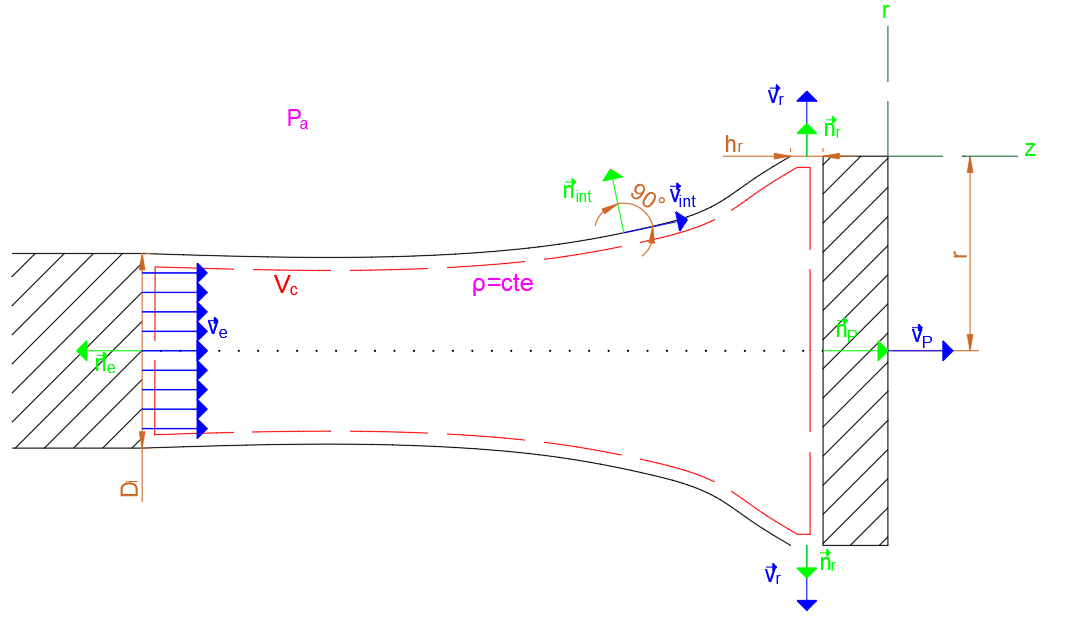
\includegraphics[width=0.7\linewidth]{imagenesEjercicios/chorro placa}
	\caption{Esquema del problema.}
	\label{fig:depositobloqueado}
\end{figure}
\textcolor{blue}
{
	Se coloca el sistema de referencia en la placa y con velocidad $\vec{v}_p$ que como es constante no provoca fuerzas de inercia. De esta manera el chorro sale a la velocidad: $\vec{v}_e-\vec{v}_p$
	\\
	Se plantea la ecuación de conservación de la masa: 
	\[\frac{d}{dt}\iiint_{V_c}\rho\,dV+\oiint_{S_c} \rho\left[(\vec{v}-\vec{v}_c)\cdot\vec{n}\right] \,dS=0\]
	Como el volumen de control no cambia:
	\[\frac{d}{dt}\iiint_{V_c}\rho\,dV=0\]
	Desarrollando el término de superficie:
	\[\oiint_{S_c} \rho\left[(\vec{v}-\vec{v}_c)\cdot\vec{n}\right] \,dS=\]
	\[
	\iint_{S_e} \rho\left[(\vec{v}-\vec{v}_c)\cdot\vec{n}\right] \,dS
	+
	\iint_{S_{int}} \rho\left[(\vec{v}-\vec{v}_c)\cdot\vec{n}\right] \,dS
	+
	\iint_{S_r} \rho\left[(\vec{v}-\vec{v}_c)\cdot\vec{n}\right] \,dS
	+
	\iint_{S_P} \rho\left[(\vec{v}-\vec{v}_c)\cdot\vec{n}\right] \,dS
	\]
	La velocidad del volumen de control $\vec{v}_c=0$
	\begin{itemize}
		\item En la salida del chorro, por ser un perfil uniforme:
			\[\iint_{S_e} \rho\left[(\vec{v}-\vec{v}_c)\cdot\vec{n}\right] \,dS=
			\iint_{S_e} \rho \left( v_e-v_P \right)\vec{i}\cdot-\vec{i} \,dS=
			-\left(v_e-v_P\right)\frac{\pi D^2_i}{4}\]
		\item En la interfase como la velocidad es siempre perpendicular a la superficie:
			\[\iint_{S_{int}}\rho\left[(\vec{v}-\vec{v}_c)\cdot\vec{n}\right]\,dS=0\]
		\item En la dirección radial de la placa:
			\[\iint_{S_r} \rho\left[(\vec{v}-\vec{v}_c)\cdot\vec{n}\right] \,dS=\iint_{S_r} \rho v_r\vec{e}_r\cdot\vec{e}_r \,dS=v_r2\pi r h(r) \text{[Área de un cilindro]}\]
		\item En la placa, como la velocidad del fluido es 0:
			\[\iint_{S_P} \rho\left[(\vec{v}-\vec{v}_c)\cdot\vec{n}\right]\,dS=0\]
	\end{itemize}
	Por tanto:
		\[\left(v_e-v_P\right)\frac{\pi D^2_i}{4}=v_r2\pi r h(r)\]
	Planteando la conservación de la cantidad de movimiento:
		\[\iiint_{V_c}\vec{f}_V\,dV
		+
		\oiint_{S_c}\left(-P\overline{\overline{I}}+\overline{\overline{\tau}}\right)\cdot\vec{n}\,dS=
		\iiint_{V_c}\frac{\partial \rho\vec{v}}{\partial t}\,dV
		+ \oiint_{S_c}\rho\vec{v}\left[\left(\vec{v}-\vec{v}_c\right)\cdot\vec{n}\right]\,dS\]
	Se desprecia el término de fuerzas volumétricas (número de Froude elevado):
		\[\iiint_{V_c}\vec{f}_V\,dV=0\]
	El término de fuerzas superficiales:
		\[\oiint_{S_c}\left(-P\overline{\overline{I}}+\overline{\overline{\tau}}\right)\cdot\vec{n}\,dS=\]
		\[
		\iint_{S_e}\left(-P\overline{\overline{I}}+\overline{\overline{\tau}}\right)\cdot\vec{n}\,dS
		+
		\iint_{S_{int}}\left(-P\overline{\overline{I}}+\overline{\overline{\tau}}\right)\cdot\vec{n}\,dS
		+
		\iint_{S_r}\left(-P\overline{\overline{I}}+\overline{\overline{\tau}}\right)\cdot\vec{n}\,dS
		+
		\iint_{S_P}\left(-P\overline{\overline{I}}+\overline{\overline{\tau}}\right)\cdot\vec{n}\,dS
		\]
	Aplicando el mismo razonamiento que en anteriores ejercicios se introduce la presión atmosférica $P_a$. Como el número de Reynolds y Froude son elevados porque es un líquido está dentro de un gas, $\overline{\overline{\tau}} $ es despreciable.
	\begin{itemize}
		\item En la salida del chorro, por ser un perfil uniforme y la presión es la atmosférica:
			\[\iint_{S_e}\left[-(P-P_a)\overline{\overline{I}}+\overline{\overline{\tau}}\right]\cdot\vec{n}\,dS=0\]
		\item En la interfase como la presión es la atmosférica:
			\[\iint_{S_{int}}\left[-(P-P_a)\overline{\overline{I}}+\overline{\overline{\tau}}\right]\cdot\vec{n}\,dS=0\]
		\item En la dirección radial de la placa como la presión es la atmosférica:
			\[\iint_{S_r}\left[-(P-P_a)\overline{\overline{I}}+\overline{\overline{\tau}}\right]\cdot\vec{n}\,dS=0\]
		\item En la placa:
			\[\iint_{S_p}\left[-(P-P_a)\overline{\overline{I}}+\overline{\overline{\tau}}\right]\cdot\vec{n}\,dS=-F_{jet+atm\rightarrow placa}\]
	\end{itemize}
	El término local es despreciable ya que el fluido es globalmente estacionario:
		\[\iiint_{V_c}\frac{\partial \rho\vec{v}}{\partial t}\,dV=0\]
	El término superficial, teniendo en cuenta como en los desarrollos anteriores solo eran no nulos los términos a la salida del chorro y en la dirección radial de la placa:
		\[\oiint_{S_c}\rho\vec{v}\left[\left(\vec{v}-\vec{v}_c\right)\cdot\vec{n}\right]\,dS=
		\iint_{S_e}\rho\vec{v}\left[\left(\vec{v}-\vec{v}_c\right)\cdot\vec{n}\right]\,dS
		+
		\iint_{S_r}\rho\vec{v}\left[\left(\vec{v}-\vec{v}_c\right)\cdot\vec{n}\right]\,dS\]
	\begin{itemize}
		\item En la salida del chorro:
			\[\iint_{S_e}\rho\vec{v}\left[\left(\vec{v}-\vec{v}_c\right)\cdot\vec{n}\right]\,dS=
			\iint_{S_e}\rho \left(v_e-v_p\right) \vec{k}\left[\left(v_e-v_p\right) \vec{k}\cdot-\vec{k}\right]\,dS=-\rho\left(v_e-v_p\right)^2\frac{\pi D^2_i}{4}\vec{k}\]
		\item En la dirección radial de la placa:
			\[\iint_{S_r}\rho\vec{v}\left[\left(\vec{v}-\vec{v}_c\right)\cdot\vec{n}\right]\,dS=
			\iint_{S_r}\rho v_r \vec{e}_r\left[v_r \vec{e}_r\cdot\vec{e}_r\right]\,dS=\rho v^2_r\iint_{S_r}\vec{e}_r\,dS=0 \text{ Ver figura inferior}\]
		\begin{figure}[H]
			\centering
			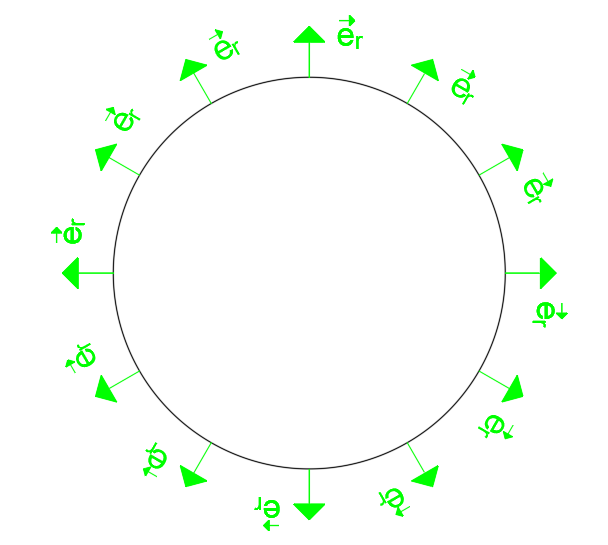
\includegraphics[width=0.6\linewidth]{imagenesEjercicios/resultante0}
			\caption{Representación de $\vec{e}_r$ a lo largo de la superficie.}
			\label{fig:resultante0}
		\end{figure}
	\end{itemize}
	Por tanto:
		\[F_{jet+atm\rightarrow placa}=\rho\left(v_e-v_p\right)^2\frac{\pi D^2_i}{4}\vec{k}\]
}
\item Dado el depósito de la Figura \ref{fig:depositoaltura}, determinar la expresión de la longitud que recorre el chorro que sale del depósito, en función del tiempo.
\begin{figure}[H]
	\centering
	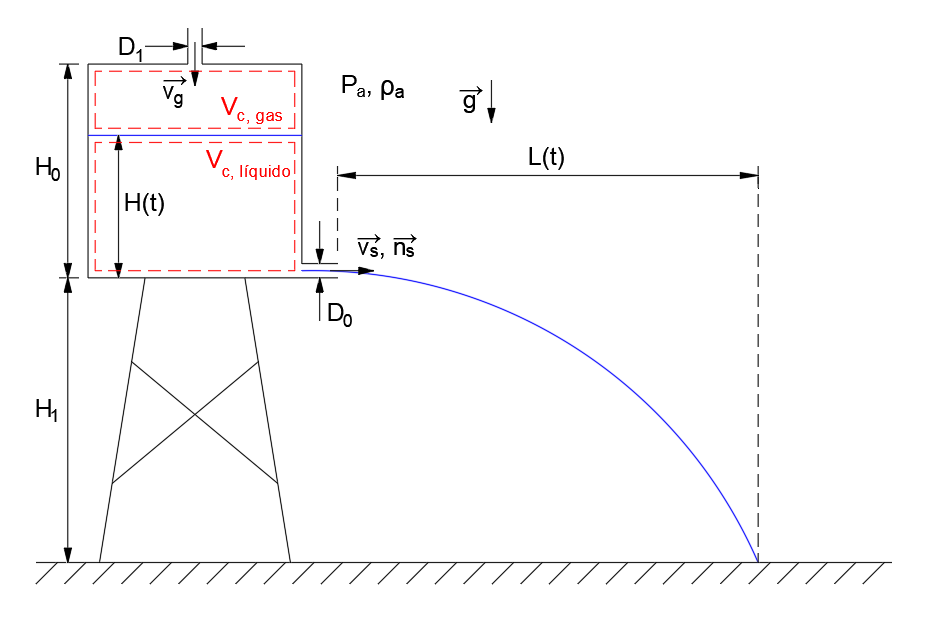
\includegraphics[width=0.9\linewidth]{imagenesEjercicios/depositoAltura}
	\caption{Esquema del depósito en altura.}
	\label{fig:depositoaltura}
\end{figure}

\blue
\textit{\textbf{Forma macroscópica.}}
\[V_C = V_{\text{depósito}} = V_{C, \text{líquido}} + V_{C, \text{gas}}\]
\[\dfrac{d}{dt} \iiint_{V_{C_l}} \rho\,dV + \oiint_{S_{C_l} = S_p \cup S_{nivel} \cup S_{salida}} \rho (\vec{v}-\vec{v}_C) \cdot \vec{n}\,dS=0\]

\begin{itemize}
	\item El término local:
	\[\dfrac{d}{dt} \iiint_{V_{C_l}} \rho\,dV = \rho A \dfrac{dH}{dt}\]
	\item El término convectivo:
	\[\oiint_{S_{C_l} = S_p \cup S_{nivel} \cup S_{salida}} \rho (\vec{v}-\vec{v}_C) \cdot \vec{n}\,dS=\rho v_s \dfrac{\pi D_0^2}{4}\]
\end{itemize}

\[-A\dfrac{dH}{dt} = v_s\dfrac{\pi D_0^2}{4}\]

\[Q_{\text{líquido}} = Q_{\text{gas}} \Rightarrow v_s\dfrac{\pi D_0^2}{4} = v_g\dfrac{\pi D_1^2}{4}\]
\[\dfrac{dV_C}{dt} = 0 \Rightarrow \dfrac{dV_{C_{\text{líquido}}}}{dt} = -\dfrac{dV_{C_{\text{gas}}}}{dt}\]

Analizando el lazo de presiones:

\[
	\begin{matrix}
		P_1 = P_a\\
		P_2 + \dfrac{1}{2}\rho_a v_g^2 = P_1 + \dfrac{1}{2}\rho_a v_{g,atm}^2\\
		P_3 = P_2(\rho_a \text{ es muy pequeña})\\
		P_4 = P_3 (\text{interfase plana})\\
		P_5 = P_4 + \rho_l g H(t)\\
		P_6 = P_5
		P_7 + \dfrac{1}{2} \rho_l v_s^2 = P_6\\
		P_7 = P_a
	\end{matrix}
\]

Donde $P_1$ es la presión antes del orificio 1 (por donde entra el gas), $P_2$ la presión después del orificio, $P_3$ antes de la interfase, $P_4$ después de la interfase, $P_5$ en el fondo del depósito, $P_6$ algo antes del orificio de salida y $P_7$ la presión tras salir del edificio.


Sabiendo que el término $\dfrac{1}{2}\rho_a v_{g,atm}^2$ es despreciable frente a $\dfrac{1}{2}\rho_a v_{g}^2$, tras sumar todas las presiones resulta:
\[\dfrac{1}{2}\rho_a v_{g}^2 = \dfrac{1}{2}\rho_a v_{s}^2 + \rho g H(t)\]

\textit{\textbf{Forma microscópica.}}


\end{enumerate}